% !TEX root = main-crime.tex

\section{Introduction}

Understanding how to control crime is important because exposures to violence and crime have been unusually high in the U.S. for several decades and, while declining, they remain high~\cite{Baum05, Fink08}. Over half a million children and youth aged 10-24 years were treated in 2012 in emergency departments for nonfatal physical assault injuries related to gun shots, cuts and stabbings, among others~\cite{cdc15}.  Understanding the neighborhood context of crime is particularly important because victimization and other forms of crime exposures have many severe consequences.  Beyond the high medical bills and violent death, consequences include behavioral and mental health problems, aggression, substance abuse, post-traumatic stress disorder, and suicide, lower academic achievement, and engaging in further violence~\cite{Grai15}. 

In this paper, we study the problem of crime rate inference of communities. We select Chicago as the target of study for the following reason. Chicago has more homicides and non-negligent manslaughter rates (15.2)
per 100,000 residents than New York (4.0) and Los Angeles (6.5)
according to the FBI crime statistics for 2013 and has experienced no
decline in the past decade compared to the other two large cities,
which have been on a slow declining slope \cite{crime-stats}.


\begin{figure}[t]
\centering
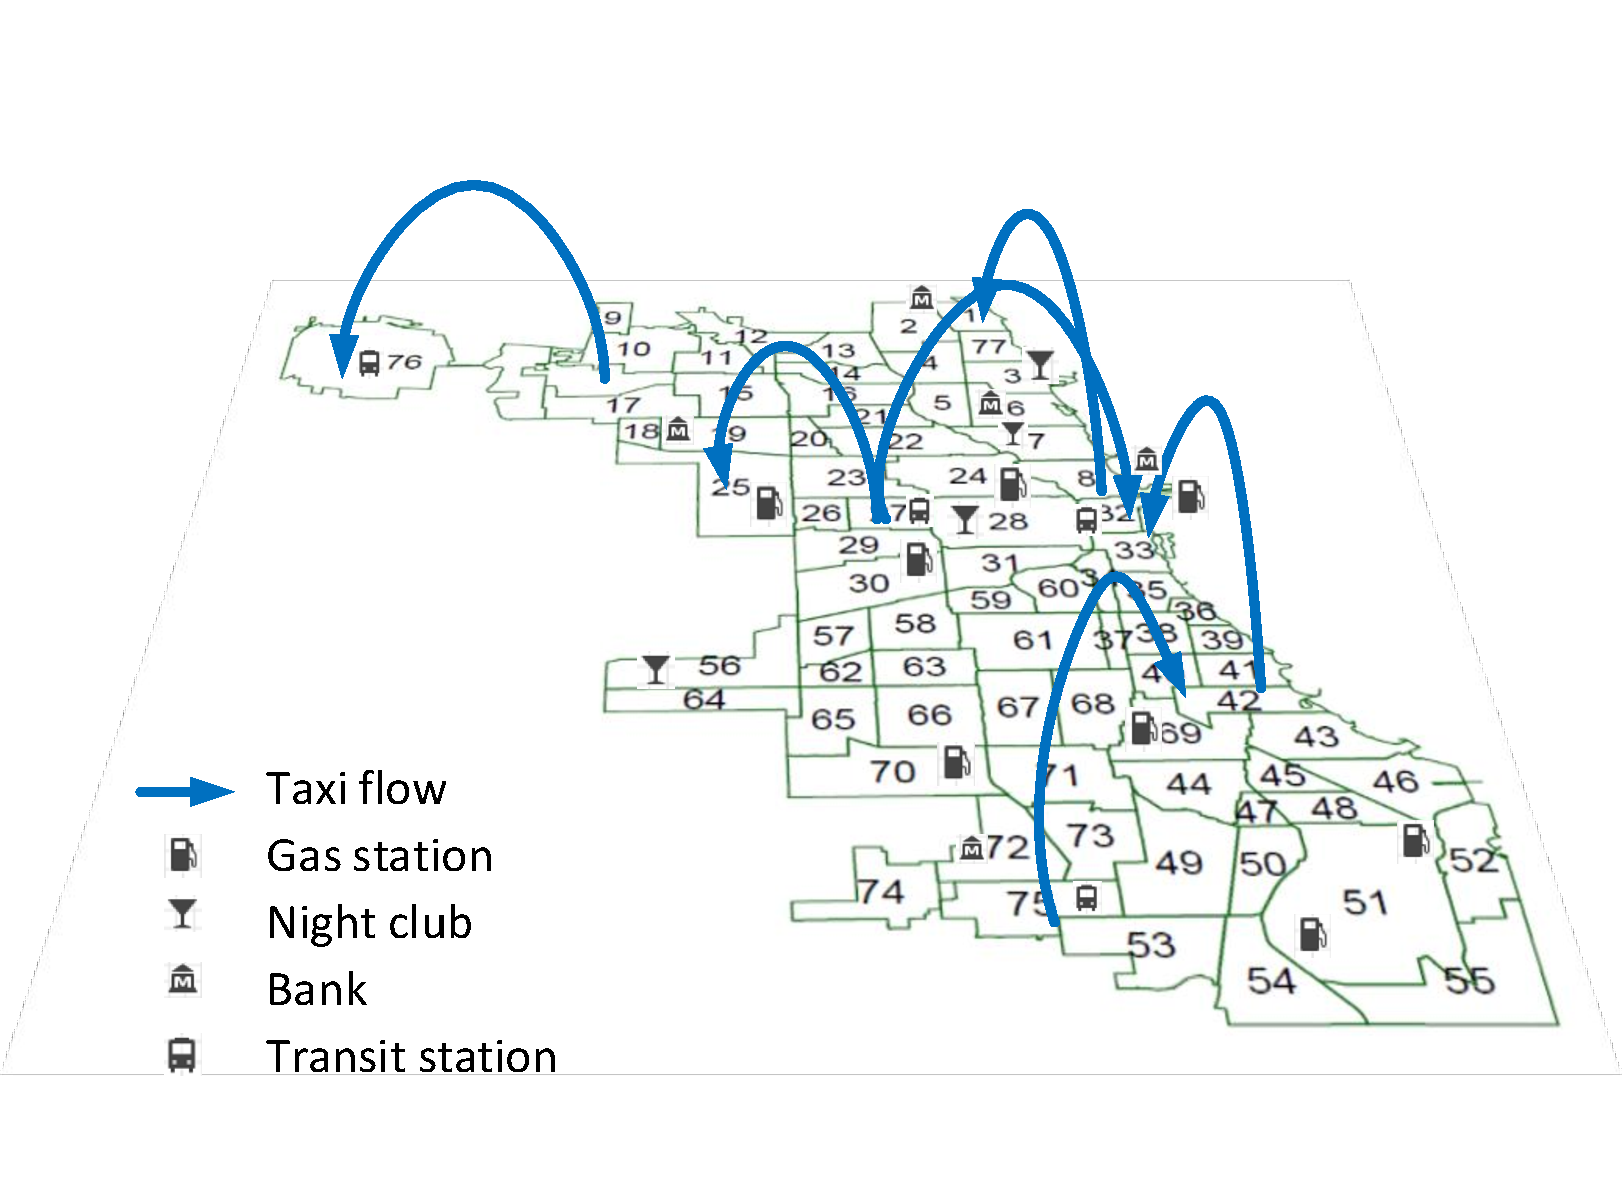
\includegraphics[width=0.7\textwidth]{fig/demo-kdd16.pdf}
\vspace{-5mm}
\caption{An illustration of various types of features we used in Chicago. The POI distribution across community areas reflects profiles of the region functionality. The taxi flow connects non-adjacent regions and act as ``hyperlinks'' on the space.}
\label{fig:demo}
\vspace{-6mm}
\end{figure}

Traditionally, researchers have used demographic information (e.g., population poverty level, socioeconomic disadvantage, racial composition of population) to estimate the crime rate in a community~\cite{GrSa09}. However,  such demographic information only contains partial information about the neighborhoods and does not dynamically reflect the changes in the community (e.g., official counts are collected by the U.S. Census Bureau every 10 years). Using only demographic information will result in a relative error of at least 30\% for crime rate estimation in Chicago (refer to experiment section in the paper). Existing studies also use the geographical influence~\cite{Ans02} to estimate the crime rate, i.e., the crime in the nearby communities can be propagated to the focal community. But this geographical influence is of little help in improving the crime inference on top of demographic feature, with at most 0.4\% relative improvement in our experiments. This is probably because the nearby communities also share similar demographics, which limits the additional benefit of geographical influence.



Recently, big data reflecting city dynamics have become widely available~\cite{ZCWY14}, e.g., traffic flow, human mobility, social media, and crowd-generated Points-Of-Interest (POI). As shown in Figure~\ref{fig:demo}, such newer types of big data could provide us new insights to understand some traditional socioeconomic urban problems, such as the crime rate inference problem we focus on in this paper. In particular, we propose to study two newer types of urban data: POI and taxi flow. 

\textbf{POI data.} POI data provide venue information such as GPS coordinates, category, popularity, and reviews. These POIs mostly belong to categories such as food, shop, transit, education, etc. Recent studies have shown that using such categorical information of POIs are useful to profile neighborhood functions~\cite{YZX12}. Such neighborhood functions could further help us predict crime rate (e.g., communities with less education or entertainment facilities may have a higher rate of crime). Our experiments show that incorporating POI features   significantly improve the crime rate inference. Adding POI features in addition to demographics features reduces the relative error by at least 5\% in our experiments. This demonstrates that POI data provide additional information about the communities that is not covered by the demographics.

\textbf{Taxi flow data.} A huge amount of taxi flow data reflect how people commute in the city. In previous studies, when using geographical influence~\cite{Ans02}, people assume that a community is affected by the spatially nearby communities. However, communities are not only affected by spatially-close communities. Even if two communities are distant in geographical space, they could have a strong correlation if many people frequently travel between these two communities~\cite{GGM14}. We hypothesize that taxi flows may be considered as ``hyperlinks'' in the city that connect the locations and we use such data to estimate crime rates. 
Taxis may be preferred to public transportation by offenders traveling to a crime location as they offer more privacy and more flexible pick-up and drop-off points. Even if taxis do not constitute the main transportation mode in committing crime, taxi flows may be a proxy for broader patterns of population routine activity and mobility, commuting flows, and other forms of social and economic exchanges between two communities over space. Such exchanges may  increase the number of potential targets and opportunities for crime \cite{CLFM79,BPBP95} or contribute to inter-community diffusion of information about successful local strategies to control  or prevent crime (e.g., successful features of neighborhood watch programs). Our experiments show very promising results --  adding taxi flow data on top of all other features can further decrease the error by 5\%.

We conduct extensive experiments including a systematic comparison between linear regression and negative binomial models, tests of different combinations of  features, detailed discussions of how to construct features, analysis of the relative importance of features, and theoretical interpretations of the results from a social scientist (a co-author in the paper). The experiments are conducted on the crime data over multiple years. We demonstrate that using the big urban data shows significant improvements.

In summary, the contribution of this paper are:  1) We study an old but very important crime inference problem by utilizing new urban data: POIs and taxi flows. 2) We find that utilizing these new types of big urban data significantly improves the crime rate inference. 3) We conduct systematic experiments to compare different results and feature combinations. The significantly better performance could serve as a new baseline for future crime inference problems.

The rest of this chapter is organized as follows. We first review the related work in Section \ref{sec:related-work}. The crime inference problem is formulated in Section \ref{sec:overview}. We discuss the inference model in Section \ref{sec:model} and feature extraction procedure in Section \ref{sec:feature}. The Section \ref{sec:experiment} presents the quantitative evaluation results on real data. Finally, we conclude this chapter in Section \ref{sec:conclusion}.

